\documentclass{article}

\usepackage[utf8]{inputenc}
\usepackage{amsmath}
\usepackage{amssymb}
\usepackage{amsthm}
\usepackage{amsfonts}
\usepackage{enumerate}
\usepackage[margin=1in]{geometry}
\usepackage[colorlinks]{hyperref}
\usepackage{tikz}
\usetikzlibrary{automata, positioning, arrows, matrix}
\tikzset{->, >=stealth', node distance = 2cm}

\setlength\parindent{0pt}

\usepackage{titlesec}
\titleformat{\section}[block]
  {}{\S\thesection}{0.25cm}{\Large}
\title{Automata and Languages}
\author{Amit Rajaraman}
\date{March 2020}

\renewcommand{\qedsymbol}{$\blacksquare$}
\newcommand{\yields}{\Rightarrow}
\newcommand{\derives}{\overset{*}{\yields}}
\newcommand{\writeNPDA}{(Q,\Sigma,\Gamma,\delta,q_0,Z_0,F)}

\numberwithin{equation}{section}
\theoremstyle{definition}
\newtheorem{theorem}{Theorem}
\newtheorem{lemma}[theorem]{Lemma}
\newtheorem{corollary}[theorem]{Corollary}
\newtheorem{definition}{Definition}
\numberwithin{definition}{section}
\numberwithin{theorem}{section}
\newtheorem{exercise}{Exercise}
\newtheorem*{example}{Example}

\theoremstyle{remark}
\numberwithin{exercise}{section}
\newtheorem*{solution}{Solution}

\begin{document}
\maketitle
\tableofcontents
\clearpage

\input{sec1}

\section{Context-Free Languages}
In this chapter, we shall present context-free grammars, that can describe certain features that have a recursive structure. They naturally arise from trying to understand the relationship of terms like nouns, verbs and prepositions in ordinary grammar, and their respective phrases which lead to a natural recursion.

An important application of this is in most compilers and interpreters, which contain a parser that extracts the meaning of a program prior to compilation. A number of methods help construct this parser once a context-free language is available. Some even automatically generate the parser.

The collection of associated languages are \textit{context-free languages}.

\subsection{Context-Free Grammars}

\begin{example}
The following is a context-free grammar. Call it $G_1$.
\begin{align*}
    A &\to 0A1 \\
    A &\to B \\
    B &\to \#
\end{align*}
The grammar consists of \textit{substitution rules} or \textit{productions}. Each rule has a symbol, called a \textit{variable}, and a string separated by an arrow. The string contains variables and other symbols called \textit{terminals}. One variable is designated as the start variable, and usually occurs on the left-hand side of the top-most rule. Using a grammar, we describe a language, called a context-free language, by generating each string of that language as follows.
\begin{enumerate}
    \item Write down the start variable.
    \item Find a variable that is written down and a rule that starts with that variable. Replace that variable with the right hand side of that rule.
    \item Repeat step $2$ until no more variables remain.
\end{enumerate}
For example, $G_1$ generates $00\# 11$ as follows.
$$A\implies 0A1\implies 00A11\implies 00B11\implies 00\# 11$$
\end{example}

\bigskip
The above information may also be represented pictorially by a \textit{parse tree}.

\vspace{3mm}
In the above example, the two rules with $A$ on the left-hand side can be merged into a single rule as  $A\to 0A1\mid B$, using the symbol ``$|$" as an ``or". To understand the link with the English language, we give a more illustrative example below.
\begin{example}
\begin{align*}
    \langle\texttt{SENTENCE}\rangle &\to \langle\texttt{NOUN-PHRASE}\rangle\langle\texttt{VERB-PHRASE}\rangle \\
    \langle\texttt{NOUN-PHRASE}\rangle &\to \langle\texttt{CMPLX-NOUN}\rangle\mid\langle\texttt{CMPLX-NOUN}\rangle\langle\texttt{PREP-PHRASE}\rangle \\
    \langle\texttt{VERB-PHRASE}\rangle&\to\langle\texttt{CMPLX-VERB}\rangle\mid\langle\texttt{CMPLX-VERB}\rangle\langle\texttt{PREP-PHRASE}\rangle \\
    \langle\texttt{PREP-PHRASE}\rangle&\to\langle\texttt{PREP}\rangle\langle\texttt{CMPLX-NOUN}\rangle \\
    \langle\texttt{CMPLX-NOUN}\rangle&\to\langle\texttt{ARTICLE}\rangle\langle\texttt{NOUN}\rangle \\
    \langle\texttt{CMPLX-VERB}\rangle&\to\langle\texttt{VERB}\rangle\mid\langle\texttt{VERB}\rangle\langle\texttt{NOUN-PHRASE}\rangle \\
    \langle\texttt{ARTICLE}\rangle&\to\texttt{a}\mid\texttt{the} \\
    \langle\texttt{NOUN}\rangle&\to\texttt{boy}\mid\texttt{girl}\mid\texttt{flower} \\
    \langle\texttt{VERB}\rangle&\to\texttt{touches}\mid\texttt{sees}\\
    \langle\texttt{PREP}\rangle&\to\texttt{with}
\end{align*}

Strings in this grammar include\\
\quad \texttt{a boy sees} \\    
\quad \texttt{the boy touches a flower} \\
\quad \texttt{the girl touches the boy with the flower}
\end{example}

\begin{exercise}
Show two different ways in which the third string in the above grammar can be generated. Here, ``two different ways" means two different parse trees, not two different derivations. (Why aren't these two the same?) Note the correspondence between these two ways and the two ways the string can be read.
\end{exercise}

\vspace{3mm}
Let us formalize our definition of a context-free grammar.
\begin{definition}
A \textit{context-free grammar} is a $4$-tuple $(V,\Sigma,R,S)$, where
\begin{enumerate}
    \item $V$ is a finite set called the \textit{variables}.
    \item $\Sigma$ is a finite set, disjoint from $V$, called the \textit{terminals}.
    \item $R$ is a finite set of \textit{rules}, with each rule being a variable and a string of variables and terminals. More precisely, $R$ is a finite subset of $V\times (V\cup\Sigma)^*$, called the \textit{set of rules}.
    \item $S\in V$ is the \textit{start variable}.
\end{enumerate}
\end{definition}

We shall abbreviate ``context-free grammar" as CFG and ``context-free language" as CFL.

If $u,v$ and $w$ are strings of variables and terminals, and $A\to w$ is a rule of the grammar, we say that $uAv$ \textit{yields} $uwv$, written as $uAv\yields uwv$.

We say that $u$ \textit{derives} $v$, written $u\derives v$, if $u=v$ or there is a sequence $u_1,u_2,\ldots,u_k$ of strings of terminals and variables exists for $k\geq 0$ such that $$u\yields u_1\yields u_2 \yields\cdots\yields u_k\yields v$$

The \textit{language} of the grammar is $\{w\in\Sigma^*\mid S\derives w\}$.

\begin{exercise}
Put the two examples given above in the form given in the definition of a CFG.
\end{exercise}

Many CFLs are the union of simpler CFLs. These can then easily be combined to form a corresponding CFG by combining their rules and then adding a new rule $S\to S_1\mid S_2\mid\cdots\mid S_k$, where the $S_i$s are the start variables of each of the CFGs.

\begin{exercise}
Construct a CFG which has corresponding language $\{0^n1^n\mid n\geq 0\}\cup\{1^n0^n\mid n\geq 0\}$
\end{exercise}
\begin{solution}
We can combine the two following CFGs:
$$S_1\to 0S_11\mid\varepsilon \text{ and } S_2\to 1S_20\mid\varepsilon$$
to get a grammar that generates the given language as follows.
\begin{align*}
    S&\to S_1\mid S_2 \\
    S_1&\to 0S_11\mid\varepsilon \\
    S_2&\to 1S_20\mid\varepsilon
\end{align*}
\end{solution}

\begin{theorem}
Any regular language is a context-free language.
\end{theorem}
\begin{proof}
Let $N(Q,\Sigma,\delta,q_0,F)$ be a DFA that recognizes the given regular language. We convert $N$ to a CFG $G(V,\Sigma,R,S)$ as follows.
\begin{itemize}
    \item $V=Q$
    \item $R=\{q_i\to aq_j\mid q_i,q_j\in V \text{ and } \delta(q_i,a)=q_j\} \cup\{q_i\to\varepsilon\mid q_i\in F\}$
    \item $S=q_0$
\end{itemize}
We leave it to the reader to verify that this grammar generates the language that the DFA recognizes.
\end{proof}

If a grammar generates a string in multiple ways, we say that the string is generated ambiguously from the grammar.
\begin{definition}
A derivation of a string $w$ in a grammar $G$ is a \textit{leftmost derivation} if at every step the leftmost remaining variable is replaced.
\end{definition}

\begin{definition}
A string $w$ is derived \textit{ambiguously} in a context-free grammar $G$ if it has two or more different left-most derivations. Grammar $G$ is \textit{ambiguous} if it generates some string ambiguously.
\end{definition}

Sometimes when we have an ambiguous grammar, we can find an unambiguous grammar that generates the same language. Some languages, however, can only be generated by ambiguous grammars. Such languages are called \textit{inherently ambiguous}.

\vspace{3mm}
It is often very useful to represent context-free grammars in a simplified form.

\begin{definition}
A context-free grammar is in \textit{Chomsky normal form} if every rule is of the form
\begin{align*}
    A&\to BC \\
    A&\to a
\end{align*}
where $a$ is any terminal, $A$ is any variable and $B,C$ are any variable other than the start variable. In addition, we permit the rule $S\to\varepsilon$, where $S$ is the start variable.
\end{definition}

\begin{theorem}
Any context-free language can be generated by a context-free grammar in Chomsky normal form.
\end{theorem}
\begin{proof}
We can convert any CFG $G$ into Chomsky normal form as follows.

\begin{enumerate}
    \item Add a new variable $S_0$ and the rule $S_0\to S$, where $S$ was the original start variable. This is done to ensure that the start variable is not on the right side of any rule.
    \item Next, we take care of all $\varepsilon$-rules, that is, rules with $\varepsilon$ on the right side. We remove any $\varepsilon$-rule $A\to\varepsilon$, where $A\neq S$. Then for each occurrence of $A$ on the right side of a rule, we add a new rule with that occurrence deleted. We repeat this until there are no $\varepsilon$ rules not involving $S$.
    \item We then handle all unit rules. We remove a unit rule $A\to B$. Then wherever a rule $B\to u$ appears, we add the rule $A\to u$ unless this was a unit rule previously removed. Here, $u$ is a string of variables and terminals. We repeat this until there are no unit rules.
    \item Given any rule $A\to u_1u_2\cdots u_k$, where $k>2$ and each $u_i$ is a variable or terminal symbol, with the rules $A\to u_1A_1, A_1\to u_2A_2, \ldots,$ and $A_{k-2}\to u_{k-1}u_k$ (The $A_i$s  are new variables).
    \item Finally, if we have any rule $A\to u_1u_2$, we replace any terminal $u_i$ with the new variable $U_i$ and add the rule $U_i\to u_i$.
\end{enumerate}

It can be checked that the language of this grammar is the same as that of the original grammar.
\end{proof}

\begin{exercise}
Convert to the following CFG to Chomsky normal form.
\begin{align*}
    S&\to ASA\mid aB \\
    A&\to B\mid S \\
    B&\to b\mid\varepsilon
\end{align*}
\end{exercise}
\begin{solution}
Performing the algorithm given in the above proof yields the following CFG.
\begin{align*}
    S_0&\to AA_1\mid UB\mid a\mid SA\mid AS \\
    S&\to AA_1\mid UB\mid a\mid SA\mid AS \\
    A&\to b\mid AA_1\mid UB\mid a\mid SA\mid AS \\
    A_1&\to SA \\
    U&\to a \\
    B&\to b \\
\end{align*}
\end{solution}
\clearpage

\subsection{Pushdown Automata}
We shall now introduce another computational model called a \textit{pushdown automaton}. These automata are like DFAs, but they have an extra component called a \textit{stack}, which provides additional memory beyond that of just the DFA. This allows the automaton to recognize certain non-regular languages. Pushdown automata are equivalent in power to context-free grammars. 

The schematic of a finite automaton can be understood as follows:
\begin{center}
\begin{tikzpicture}[block_center/.style ={rectangle, draw=black, fill=white, text width=7em, text centered, minimum height=4em}, cell/.style={rectangle,draw=black},
space/.style={minimum height=1.5em,matrix of nodes,row sep=-\pgflinewidth,column sep=-\pgflinewidth,column 1/.style={font=\ttfamily}},text depth=0.5ex,text height=2ex,nodes in empty cells]
    \node[block_center] (control) {state control};
    
    \matrix (input) [space, below right=0.2cm and 3cm of control, column 1/.style={nodes={cell,minimum width=2em}},column 2/.style={nodes={cell,minimum width=2em}},column 3/.style={nodes={cell,minimum width=2em}},column 4/.style={nodes={cell,minimum width=2em}}]
    {
    a & b & b & a \\};
    
    \node[below=0.1cm of input] {input};
    \draw (control.15) -| (input-1-1);
    \end{tikzpicture}
\end{center}

The ``state control" represents the states and the transition function, and the tape contains the input string, which is read character by character. The arrow points at the next character to be read.

\vspace{3mm}
Similarly, a pushdown automaton can be understood as follows.

\begin{center}
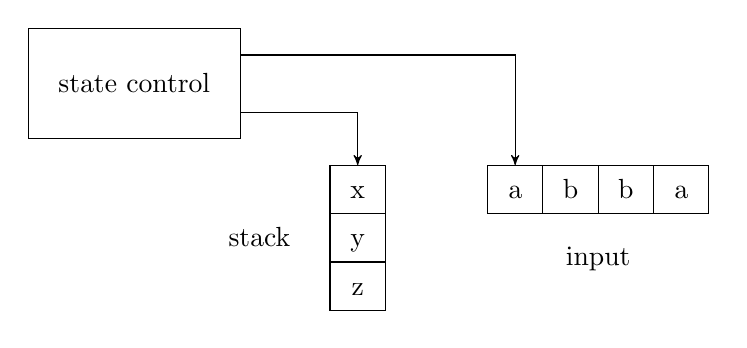
\begin{tikzpicture}[block_center/.style ={rectangle, draw=black, fill=white, text width=7em, text centered, minimum height=4em}, cell/.style={rectangle,draw=black},
space/.style={minimum height=1.5em,matrix of nodes,row sep=-\pgflinewidth,column sep=-\pgflinewidth,column 1/.style={font=\ttfamily}},text depth=0.5ex,text height=2ex,nodes in empty cells]
    \node[block_center] (control) {state control};
    
    \matrix (input) [space, below right=0.2cm and 3cm of control, column 1/.style={nodes={cell,minimum width=2em}},column 2/.style={nodes={cell,minimum width=2em}},column 3/.style={nodes={cell,minimum width=2em}},column 4/.style={nodes={cell,minimum width=2em}}]
    {
    a & b & b & a \\};
    
    \matrix (stack) [space, below right=0.2cm and 1cm of control, column 1/.style={nodes={cell,minimum width=2em}}]
    {
    x \\ y \\ z \\};

    \node[left=0.25cm of stack] {stack};
    \node[below=0.1cm of input] {input};
    \draw (control.15) -| (input-1-1);
    \draw (control.-15) -| (stack-1-1);
\end{tikzpicture}
\end{center}

In addition to the finite automaton-like structure it has, it also has a stack on which which symbols can be written down and read back later (The concept of a stack is hopefully familiar to the reader). This stack, which has infinite memory, is what enables the pushdown automaton to recognize languages such as $\{0^n1^n\mid n\geq 0\}$ because it can store the number of $0$s it has seen on the stack. The ``pushdown" in pushdown automaton corresponds to the stack structure.

\vspace{3mm}
Unlike DFAs and NFAs, deterministic pushdown automata and nondeterministic pushdown automata are \textit{not} equivalent. However, as nondeterministic pushdown automata are equivalent to context-free grammars, we shall focus on them for the remainder of this subsection.

\begin{example}
\label{LwwRexample}
Let us attempt to construct the pushdown automaton corresponding to the language $L$ described in \ref{LwwR}. We do so as follows.
\begin{itemize}
    \item Start in a state $q_0$ that represents a guess that we have not yet seen the end of the $w$ in the definition of $L$. While in state $q_0$, we read symbols and push them onto the stack.
    \item At any time, we may guess that we have reached the end of $w$. Since the automaton is nondeterministic, we guess that we have reached the end of $w$ by going to state $q_1$, and also stay in $q_0$ and continue to read inputs.
    \item Once in state $q_1$, we look at the input symbol and compare it to the topmost symbol on the stack. If they are the same, we pop it. Otherwise, the branch dies.
    \item If we empty the stack, then we have seen something of the form $ww^\mathcal{R}$, so we accept.
\end{itemize}
\end{example}

\vspace{3mm}
We shall now formally define a nondeterministic pushdown automaton.
\begin{definition}
A \textit{nondeterministic pushdown automaton} is a $7$-tuple $(Q,\Sigma,\Gamma,\delta,q_0,Z_0,F)$ where $Q,\Sigma, \Gamma, F$ are all finite sets, and
\begin{enumerate}
    \item $Q$ is the (finite) \textit{set of states},
    \item $\Sigma$ is the (finite) \textit{input alphabet},
    \item $\Gamma$ is the (finite) \textit{stack alphabet} (this is the set of elements we can push onto the stack),
    \item $\delta:Q\times\Sigma_\varepsilon\times\Gamma\to\mathcal{P}(Q\times\Gamma^*)$ is the \textit{transition function},
    \item $q_0\in Q$ is the \textit{start state},
    \item $Z_0\in\Gamma$ is a particular symbol called the \textit{start symbol}, which initially appears on the stack, and
    \item $F\subseteq Q$ is the \textit{set of accept states}.
\end{enumerate}
\end{definition}

\vspace{2mm}
We shall abbreviate ``Nondeterministic Pushdown Automaton" as NPDA.

In the above definition, the transition function is the main thing that is different from our usual definition of an NFA. In one transition, it:
\begin{enumerate}
    \item consumes from input the symbol used in the transition (if the symbol is $\varepsilon$, then no input is consumed),
    \item goes to a new state, and
    \item replaces the string at the top of the stack with a string. Note that the string could also be $\varepsilon$, which means that we pop the stack.
\end{enumerate}
Given this, the correspondence to the above definition is clear.

We require $Z_0$ in the above definition of a stack so that we can know when the stack is empty. Note that it is equivalent to use a specific symbol that we push in the beginning to signify the bottom of the stack. Some textbooks use this definition of the NPDA instead. We shall now define what it means for an NPDA to recognize a string.

\begin{definition}
An NPDA $M=\writeNPDA$ is said to \textit{accept} a string $w$ if $w$ can be written as $w=w_1w_2\cdots w_m$, where each $w_i\in\Sigma_\varepsilon$ and sequence of states $r_0,r_1,\ldots,r_m\in Q$ and strings $s_0,s_1,\ldots,s_m\in\Gamma^*$ exist that satisfy the following three conditions.
\begin{enumerate}
    \item $r_0=q_0$ and $s_0=Z_0$.
    \item For $i=0,1,\ldots,m-1$, we have $(r_{i+1},b)\in\delta(r_i,w_{i+1},a)$, where $s_i=at$ and $s_{i+1}=bt$ for some $a\in\Gamma$ and $b,t\in\Gamma^*$.
    \item $r_m\in F$.
\end{enumerate}
\end{definition}

\begin{exercise}
\label{LwwRexercise}
Express \ref{LwwRexample} in the form given in the definition of an NPDA. 
\end{exercise}
\begin{solution}
The PDA can be expressed as $P=(\{q_0,q_1,q_2\}, \{0,1\}, \{0,1,Z_0\}, \delta, q_0,Z_0, \{q_2\})$, where
\begin{align*}
    \delta(q_0,a,Z_0) &= \{(q_0,aZ_0)\}\quad\text{for all $a\in\{0,1\}$} \\
    \delta(q_0,a,b) &= \{(q_0,ab)\}\quad\text{for all $a,b\in\{0,1\}$} \\
    \delta(q_0,\varepsilon,a) &= \{(q_1,a)\}\quad\text{for all $a\in\{0,1,Z_0\}$} \\
    \delta(q_1,a,a) &= \{(q_1,\varepsilon)\}\quad\text{for all $a\in\{0,1\}$} \\
    \delta(q_1,\varepsilon,Z_0) &= \{(q_2,Z_0)\}
\end{align*}
\end{solution}

\vspace{3mm}
Similar to how we express NFAs and DFAs as graphs, NPDAs can also be expressed as graphs, where in addition to the way we draw the NFA structure, we also write what happens to the stack as follows. An arc labelled $a,X/\alpha$ from state $q$ to $p$ means that $(p,\alpha)\in\delta(q,a,X)$. That is, it tells what input is used ($a$), and the old and new tops of the stack ($X$ and $\alpha$ respectively).

\vspace{3mm}
So for instance, the PDA described in \ref{LwwRexercise} is depicted by the following diagram.

\begin{center}
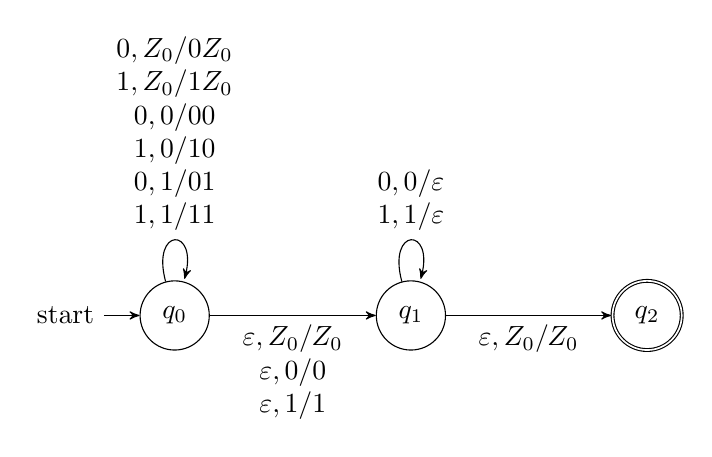
\begin{tikzpicture}[node distance=3cm]
    \node[state,initial] (q0) {$q_0$};
    \node[state,right of=q0] (q1) {$q_1$};
    \node[state,accepting,right of=q1] (q2) {$q_2$};
    \draw (q0) edge[loop above] node[align=center] {$0,Z_0/0Z_0$ \\ $1,Z_0/1Z_0$        \\ $0, 0/00$ \\ $1, 0/10$ \\ $0, 1/01$ \\ $1, 1/11$} (q0)
          (q1) edge[loop above] node[align=center]{$0, 0/\varepsilon$ \\ $1, 1/\varepsilon$} (q1)
          (q0) edge[below] node[align=center] {$\varepsilon, Z_0/Z_0$ \\ $\varepsilon, 0/0$ \\ $\varepsilon, 1/1$} (q1)
          (q1) edge[below] node[align=center] {$\varepsilon, Z_0/Z_0$} (q2);
\end{tikzpicture}
\end{center}

\begin{exercise}
Construct the NPDA that recognizes the language $L=\{a^ib^jc^k\mid i=j\text{ or }j=k\}$
\end{exercise}

It is also useful to represent a PDA at some point of time by a triple $(q,w,\gamma)$, where $q$ is the state, $w$ is the remaining input, $\gamma$ is the stack contents. We conventionally show that top of the stack at the left end of $\gamma$. Such a triple is called an \textit{instantaneous description}, or ID of the automaton.

\vspace{3mm}
Let $V=\writeNPDA$ be an NPDA. Define $\vdash_P$, or just $\vdash$ when $P$ is understood, as follows. Suppose $(p,\alpha)\in\delta(q,a,X)$. Then for all strings $w\in\Sigma^*,\beta\in\Gamma^*$, we write
$$(q,aw,X\beta)\vdash(p,w,\alpha\beta)$$
This notation, called the \textit{``turnstile"} notation, represents the transition between different IDs of the NPDA. Note that $w$ and $\beta$ do not influence the transition, they are merely carried along.

We also use $\vdash^*_P$ or $\vdash^*$ to represent $0$ or more moves of the NPDA. That is, $I\vdash^* I$ for any ID $I$ and $I\vdash J$ if there exists a state $K$ such that $I\vdash K$ and $K\vdash^* J$.

\vspace{3mm}
We shall call a sequence of IDs a \textit{computation}. We have the following.
\begin{itemize}
    \item If a computation is legal, then the computation formed by adding the same additional input string to the end of the input in each ID is also legal.
    \item If a computation is legal, then the computation formed by adding the same additional string below the stack of each ID is also legal.
    \item If a computation is legal, and some tail of the input is not consumed, we can remove this tail from each ID and the resulting computation will still be legal.
\end{itemize}

These three points just say that information that the NPDA does not look at does not affect its computation.

\begin{theorem}
If $P=\writeNPDA$ is an NPDA and $(q,x,\alpha)\vdash^*_P(p,y,\beta)$, then for any strings $w\in\Sigma^*, \gamma\in\Gamma^*$, $$(q,xw,\alpha\gamma)\vdash^*_P(p,yw,\beta\gamma).$$
\end{theorem}
\begin{proof}
This proof is trivial and is left as an exercise to the reader. (Perform an induction on the number of steps in the sequence of IDs)
\end{proof}

Using this notation, we can alternatively formulate the definition of the language recognized by a language as follows.
Let $P=\writeNPDA$ be an NPDA. Then
$$L(P)=\{(q_0,w,Z_0)\vdash^*_P(q,\varepsilon,\alpha)\mid q\in F\text{ and }\alpha\in\Gamma^*\}$$
The above condition is called \textit{acceptance by final state}, which is exactly what it is.
\begin{definition}
Let $P=\writeNPDA$ be an NPDA. We define
$$N(P)=\{w\mid (q_0,w,Z_0)\vdash^*(q,\varepsilon,\varepsilon)\}$$
\end{definition}


The above set represents the set of input strings that when consumed, empty the stack as well. This is called \textit{acceptance by empty stack}.

The following two theorems shows how the above two acceptances are intimately related.

\begin{lemma}
If $L=N(P_N)$ for some NPDA $P_N=(Q,\Sigma,\Gamma,\delta_N,q_0,Z_0)$, then there is an NPDA $P_F$ such that $L(P_F)=L$.
\end{lemma}
\begin{proof}
We first set the start symbol of $P_F$ we are creating as some $X_0\not\in\Gamma$, whose sole purpose is to let us know when we have reached the bottom of the stack. If we see $X_0$ on the stack for some input, then it means that $P_N$ would empty the stack for some input. We also set the start state of $P_F$ as some $p_0\not\in Q$, whose sole purpose is to push $Z_0$ onto the stack and send it to $q_0$. Then, $P_F$ simulates $P_N$, until the stack of $P_N$ is empty. We also create another state $p_f\not\in Q$, which is the accepting $P_F$. $P_F$ goes to $p_f$ if $P_N$ would have emptied the stack for that input (that is, it has $X_0$ on the top of the stack).

That is, $$P_F=(Q\cup\{p_0,p_f\}, \Sigma, \Gamma\cup\{X_0\}, \delta_F, p_0, X_0, \{p_F\})$$where $\delta_F$ is defined as follows.
$$
\delta_F(q,a,X)=
\begin{cases}
\{(q_0,Z_0X_0)\}\quad q=p_0, a=\varepsilon, X=X_0 \\
\delta_N(q,a,X)\quad q\in Q, a\in\Sigma_\varepsilon, X\in\Gamma \\

\end{cases}
$$
\end{proof}
\end{document}